\chapter{Mechanisms of Coronal Dimming}
\label{chaptermechanisms}



This chapter details the physics of coronal dimming. This first original contribution to the field shows that there are theoretically many physical processes that can lead to an uncareful observer identifying "dimming", which may have little to do with coronal mass ejection (CME). Traditionally, the term "coronal dimming" has been assumed to refer to the void left in the corona after a CME departs. This is one cause of a transient hole in the corona, and is of the greatest concern to space weather forecasters. Typically, a single dimming-sensitive wavelength or band will be observed and analyzed. However, changing temperatures, common during solar eruptive events, cause ionization fraction shifting, resulting in some emissions dimming while others brighten. Additionally, dark material (e.g., a filament) can pass between a bright region (e.g., flaring loops) and the observer, causing a transient dip in emission. Third, solar eruptive events sometimes have associated waves that propagate across the solar disk. These waves are observed as narrow bright fronts with a trailing dark region. The trailing dark region is another way to achieve a transient dimming of emission. Next, there are two ways that Doppler effects can cause transient dips in emission. The first is called Doppler dimming and results from fast moving plasma being sufficiently Doppler-shifted to reduce resonant fluorescence from the solar emission line sources; a phenomenon which is independent of the observation angle. The second occurs if eruptive plasma is moving fast enough in the line-of-sight to shift its emissions outside the bandpass of an observing instrument, which we have named "bandpass shift dimming". The physics, instrument effects, and mitigation strategies for each of these types of theoretically observable dimming are summarized in Table \ref{tablesummary} and are discussed in detail in the sections that follow. 

\begin{table}[!htb]
    \caption{Summary of physical processes that can manifest as observed dimming}
    \begin{center}
    \begin{tabular}{|p{2.5cm}|p{4cm}|p{4cm}|p{4cm}|} \hline
	Short Name & Physical Process & EVE Observational Identifiers & AIA Observational Identifiers \\ \hline \hline
	Mass loss (Fig. \ref{figuremassloss}) & Ejection of emitting plasma from corona & Simultaneous intensity decrease in multiple coronal emission lines, with percentage decrease indicative of percentage mass lost & Area over and near the erupting active region (AR) darkens \\ \hline
	
	Thermal (Fig. \ref{figurethermal}) & Heating raises ionization states (e.g., a fraction of Fe IX becomes Fe X); cooling does the opposite & Heating: Emission loss in lines with lower peak formation temperatures and near simultaneous emission gain in lines with higher peak formation temperatures; vice versa for cooling & Heating: Area near AR darkens in channels with lower peak formation temperature and near simultaneous brightening in channels with higher peak formation temperatures; vice versa for cooling \\ \hline
	
	Obscuration (Fig. \ref{figureobscuration}) & Dim feature (e.g., filament material) moves into line-of-sight over a bright feature (e.g., flare arcade) & Drop of emission lines proportional to their absorption cross section in the obscuring material & Direct observation of this obscuration process \\ \hline
	
	Wave (Fig. \ref{figurewave}) & Wave disturbance propagates globally, causing compression/rarefaction of plasma as wave passes by & No effects have been identified & Direct observation of this wave process, especially apparent with difference movies \\ \hline
	
	Doppler & Fast moving plasma Doppler shifts away from resonant fluorescence with solar emission lines & Doppler wavelength shift of emission lines and change in intensity, possibly also observed as line broadening & Change in intensity of moving plasma as its velocity changes \\ \hline
	
	Bandpass & Emissions from fast moving plasma have Doppler wavelength shift & Emission line shifts in wavelength or has broadening & Doppler shift convolves with band-pass sensitivity to cause apparent reduction in emission \\ \hline
	
	\end{tabular}
    \\ \rule{0mm}{5mm}
\end{center}
\label{tablesummary}
\end{table}

\section{Thermal Dimming}
(more text here + 2 figures + 2nd figure needs update)
Temperature evolution of emission lines is only interpreted as observed dimming if one is not careful to observe co-spatial emission lines at different peak formation temperatures. These "heat wave dimmings" were documented by   \citet{Robbrecht2010}. As plasma is heated or cooled, the ionization fraction changes, necessarily causing the emission intensity to change (Figure 2). For example, heating causes some Fe IX to become Fe X and thus, in the absence of competing physical processes, 171 Å emission drops while 177 Å rises. This pattern was identified observationally in Figure 6 of \citet{Woods2011}. It can also be observed in the standard composite (multi-wavelength) movies produced by the AIA team; indeed, this is one of the prime purposes for the composites. The initiation time and duration of temperature evolution tends to be quite similar to mass-loss dimming, as they are typically both responses to the rapid release of magnetic field energy in active regions and require several hours of recovery time. Thus, thermal processes could be mistaken for mass loss if only a single spectral line was observed. Ideally, unblended emission lines from an entire coronal ionization sequence (e.g., Fe I to Fe XVIII) could be used to mitigate this convolution of dimming observations. However, as we will show in Section 4.3, it may be sufficient to have observations of two sufficiently separated ionizations states to differentiate between thermal evolution and mass-loss dimming. This is due, in part, to the fact that hotter lines (e.g., Fe XV and above) are primarily emitted from confined loops near the flare and are thus not strongly impacted by mass-loss dimming. 

It is important to note that, in general, the magnitude of total observed dimming in a given line in EVE spectra is inversely proportional to its peak formation temperature, which can be inferred from Figure 3. This figure was generated using a simple algorithm that searched the EVE catalog for relative irradiance decreases greater than a specified threshold (1\%, 2\%, 3\%) after flares exceeding GOES X-ray class of C1. The window of time searched was bounded by the GOES event start time and the sooner of either 4 hours after the start time or the next GOES event start time. This algorithm was applied to all EVE data from mission start to 23 September 2013. Figure 3 shows that the number of dimmings dramatically decreases as the magnitude threshold is increased, and decreases slightly with higher peak formation temperature. This latter effect is due to flare heating adding emission in the higher temperature, higher ionization state, lines that partially offsets the mass-loss dimming. These trends indicate that at sufficiently high peak formation temperature, no dimming may be observed at all, even at the lowest detection threshold, which is consistent with the hotter lines being restricted to the confined flare loops and hence experiencing no mass loss. 

\section{Obscuration Dimming}

\section{Wave Dimming}

\section{Two Possible but Unobserved Dimming Mechanisms}

\section{Mass-loss Dimming}



Figure \ref{xfigDiagram} shows an image from a PDF file
imported into this document
using the \verb2graphicx2 package.
The command \verb2\usepackage{graphicx}2, which appears
near the very top of the main \LaTeX{} file, reads in
this package which defines the
\verb2\includegraphics{}2 macro.


\begin{figure}[htbp]
	\caption[Cylinder and measurements]{
	This diagram of a cylinder and various
	measurements and quantities was actually
	made using {\bf xfig}, a freeware
	drawing program for Unix systems.
	Diagrams can be exported directly to PDF
	files, the preferred format for
	vector graphics.  Vector graphics can
	be magnified indefinitely without degradation,
	whereas bitmap images (JPG and PNG)
	must be pretty high-resolution if you don't
	want them looking all pixellated when
	magnified.
	}
    \begin{center}
	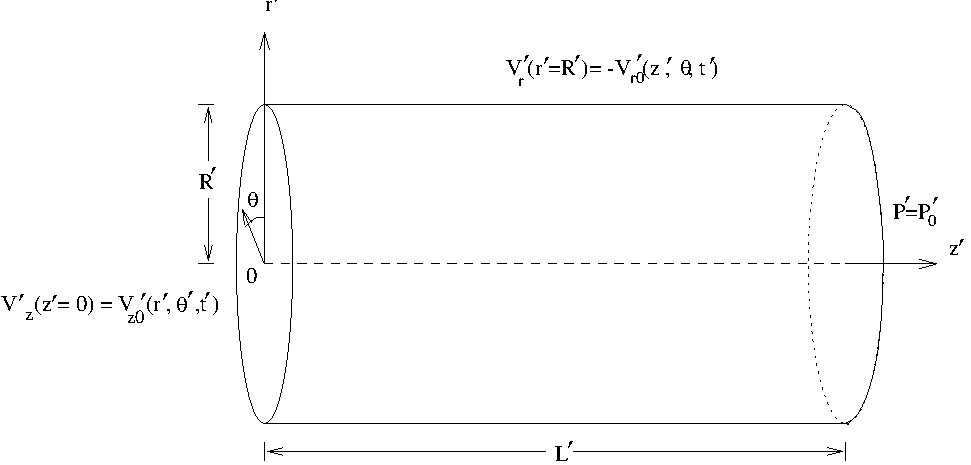
\includegraphics[width=100mm]{figs/cyl.pdf}
    \end{center}
\label{xfigDiagram}
\end{figure}